\documentclass[runningheads]{llncs}
% This is samplepaper.tex, a sample chapter demonstrating the
% LLNCS macro package for Springer Computer Science proceedings;
% Version 2.20 of 2017/10/04
%
%

\usepackage{templates/mainpreambel}

\newcommand{\attention}[1]{\color{red}\textbf{[#1]}\color{black}\unskip}
\newcommand{\xixi}[1]{\color{green}\textbf{[#1]}\color{black}\unskip}
\newcommand{\OR}[1]{\color{red}\textbf{[OR]}\color{black}\unskip}
\newcommand{\optional}[1]{\color{blue}\textbf{~#1}\color{black}\unskip}
\newcommand*{\myenquote}[1]{\enquote{{\itshape#1}}}

\newcommand{\needsciteempty}{CITE}
\newcommand{\needscitecomment}[1]{#1}
% \newcommand{\needscite}[1]{\color{purple}\textbf{\textsuperscript{
%             CITE #1
%         }}\color{black}\ignorespacesafterend}

\newcommand{\unsure}[1]{ (\color{orange} CHECK\color{black}~#1)}
% \newcommand{\conditional_probability}[2]{p\left(#1 \mid #2\right)}
\newcommand{\cprob}[2]{p\left(#1 \mid #2\right)}

\newcommand{\needsfigure}[2]{
    \begin{figure}[htb]
        \centering
        
\includegraphics[width=0.25\textwidth]{figures/misc/placeholder.png}
        \caption{#2}
        \label{#1}
    \end{figure}
}

\newcommand{\needsequation}[1]{
    \begin{align}
        \label{#1}
        someformula & = 4*2 \\
        anotherformula & = 1*3*3*7
    \end{align}
}

\newcommand{\needscite}[1]{
    \color{purple}
    \ifthenelse{\equal{#1}{}}{\textsuperscript{CITE}}{\textsuperscript{CITE #1}}
    \color{black}\ignorespacesafterend\noindent
}
\newcommand{\needsalg}[2]{
    \begin{figure}[htb]
        \centering
        
\includegraphics[width=0.25\textwidth]{figures/misc/placeholder.png}
        \caption{#2}
        \label{#1}
    \end{figure}
}
    % \begin{algorithm}
    %     \label{#1}
    %     \caption{#2}
    %     \begin{algorithmic}
    %     \Require{Write here the required data}
    %     \Ensure{Write here the expected result}
    %      \State initialization;
    %      \While{While condition}
    %       \State instructions;
    %       \If{condition}
    %        \State instructions1;
    %        \State instructions2;
    %       \Else
    %        \State instructions3;
    %       \EndIf
    %      \EndWhile
    %     \end{algorithmic}
    % \end{algorithm}    

\newenvironment{optional*}[1][]
{
    \noindent
    \color{blue}
    \textit{OPTIONAL\ifthenelse{\isempty{#1}}{}{#1}:}
}
{
    \color{black}
}

\newcommand{\nullvector}{
    \mathbf{0}
}
\newcommand{\cProbCurrState}{\cprob{z_t}{t, z_{1:T}, u_{t}, \theta_h}}
\newcommand{\cProbNextState}{\cprob{z_{t+1}}{t, z_{1:T}, u_{1:T}, x_{1:T}, \theta_h}}
\newcommand{\cProbCurrObservation}{\cprob{x_t}{t, z_{1:T}, u_{1:T}, \theta_g}}

\newcommand{\cProbCurrShortState}{\cprob{z_t}{z_{1:t}, u_{t}, \theta_h}}
\newcommand{\cProbNextShortState}{\cprob{z_{t+1}}{z_{1:t}, u_{1:t}, \theta_h}}
\newcommand{\cProbCurrShortObservation}{\cprob{x_t}{z_{1:t}, \theta_g}}
\newcommand{\editCost}{cost_{a_i, b_j}}
\newcommand{\editCostFunction}[2]{cost(#1, #2)}
\newcommand{\editCostFunctionNoB}{cost(a_i, \nullvector)}
\newcommand{\editCostFunctionNoA}{cost(\nullvector, b_j)}
\newcommand{\editCostFunctionBoth}{cost(a_i, b_j)}
\newcommand{\editDistance}[2]{d_{a, b}(#1, #2)}
\newcommand{\currentState}{\mathbf{z}_t}
\newcommand{\nextState}{\mathbf{z}_{t+1}}
\newcommand{\currentInput}{\mathbf{u}_t}
\newcommand{\currentEvent}{\mathbf{e}_t}



\makeglossaries
\loadglsentries[acronym]{./references/glossary.tex}

% \DeclareLanguageMapping{american}{american-apa}

% Used for displaying a sample figure. If possible, figure files should
% be included in EPS format.
%
% If you use the hyperref package, please uncomment the following line
% to display URLs in blue roman font according to Springer's eBook style:
% \renewcommand\UrlFont{\color{blue}\rmfamily}

% \loadglsentries[acronym]{./references/glossary.tex}
\graphicspath{{figures/}}


\usepackage{subfiles} 

\begin{document}
%
\title{Contribution Title\thanks{Supported by organization x.}}
%
%\titlerunning{Abbreviated paper title}
% If the paper title is too long for the running head, you can set
% an abbreviated paper title here
%
\author{First Author\inst{1}\orcidID{0000-1111-2222-3333} \and
Second Author\inst{2,3}\orcidID{1111-2222-3333-4444} \and
Third Author\inst{3}\orcidID{2222--3333-4444-5555}}
%
\authorrunning{F. Author et al.}
% First names are abbreviated in the running head.
% If there are more than two authors, 'et al.' is used.
%
\institute{Princeton University, Princeton NJ 08544, USA \and
Springer Heidelberg, Tiergartenstr. 17, 69121 Heidelberg, Germany
\email{lncs@springer.com}\\
\url{http://www.springer.com/gp/computer-science/lncs} \and
ABC Institute, Rupert-Karls-University Heidelberg, Heidelberg, Germany\\
\email{\{abc,lncs\}@uni-heidelberg.de}}
%
\maketitle              % typeset the header of the contribution
%
\begin{abstract}
The abstract should briefly summarize the contents of the paper in
15--250 words.

\keywords{First keyword  \and Second keyword \and Another keyword.}
\end{abstract}
%
%
%
% TODO: Put all the thesis content in the paper
% TODO: Change chapters to sections
% NOTE: Technical papers describe original solutions (theoretical, methodological or conceptual) in the field of IS Engineering. A technical paper should clearly describe the situation or problem tackled, the relevant state of the art, the position or solution suggested and its potential‚ as well as demonstrate the benefits of the contribution through a rigorous evaluation.
% NOTE: Limit is 16 pages


\section{Introduction}
\label{sec:intro}

\subsection{Motivation}
\label{sec:motivation}
\subfile{content/sections/sec_motivation}

\subsection{Problem Space}
\label{sec:challenges}
\subfile{content/sections/sec_challenges}



\subsection{Related Literature}
\label{sec:literature}
Many researchers have worked on counterfactuals and \Gls{PM}. 
Here, we combine the important concepts and discuss the various contributions to this thesis.
\subfile{content/sections/sec_literature}


\subsection{Research Question}
\label{sec:rq}
As we seek to make data-driven process models interpretable, we have to understand the exact purpose of this thesis. Hence, we establish the open challenges and how this thesis attempts to solve them. 
% \subfile{content/sections/sec_rq}

\subsection{Outline}
% \subfile{content/sections/sec_outline}




\section{First Section}
\subsection{A Subsection Sample}
Please note that the first paragraph of a section or subsection is
not indented. The first paragraph that follows a table, figure,
equation etc. does not need an indent, either.

Subsequent paragraphs, however, are indented.

\subsubsection{Sample Heading (Third Level)} Only two levels of
headings should be numbered. Lower level headings remain unnumbered;
they are formatted as run-in headings.

\paragraph{Sample Heading (Fourth Level)}
The contribution should contain no more than four levels of
headings. Table~\ref{tab1} gives a summary of all heading levels.

\begin{table}
\caption{Table captions should be placed above the
tables.}\label{tab1}
\begin{tabular}{|l|l|l|}
\hline
Heading level &  Example & Font size and style\\
\hline
Title (centered) &  {\Large\bfseries Lecture Notes} & 14 point, bold\\
1st-level heading &  {\large\bfseries 1 Introduction} & 12 point, bold\\
2nd-level heading & {\bfseries 2.1 Printing Area} & 10 point, bold\\
3rd-level heading & {\bfseries Run-in Heading in Bold.} Text follows & 10 point, bold\\
4th-level heading & {\itshape Lowest Level Heading.} Text follows & 10 point, italic\\
\hline
\end{tabular}
\end{table}


\noindent Displayed equations are centered and set on a separate
line.
\begin{equation}
x + y = z
\end{equation}
% Please try to avoid rasterized images for line-art diagrams and schemas. Whenever possible, use vector graphics instead (see Fig.~\ref{fig1}).

\begin{figure}
% 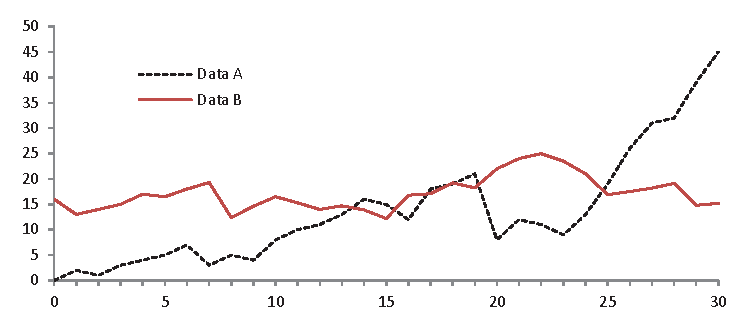
\includegraphics[width=\textwidth]{fig1.eps}
% \caption{A figure caption is always placed below the illustration. Please note that short captions are centered, while long ones are justified by the macro package automatically.} \label{fig1} 
\end{figure}

\begin{theorem}
This is a sample theorem. The run-in heading is set in bold, while
the following text appears in italics. Definitions, lemmas,
propositions, and corollaries are styled the same way.
\end{theorem}
%
% the environments 'definition', 'lemma', 'proposition', 'corollary',
% 'remark', and 'example' are defined in the LLNCS documentclass as well.
%
\begin{proof}
Proofs, examples, and remarks have the initial word in italics,
while the following text appears in normal font.
\end{proof}
For citations of references, we prefer the use of square brackets
and consecutive numbers. Citations using labels or the author/year
convention are also acceptable. The following bibliography provides
a sample reference list with entries for journal
% articles~\cite{ref_article1}, an LNCS chapter~\cite{ref_lncs1}, a
% book~\cite{ref_book1}, proceedings without editors~\cite{ref_proc1},
% and a homepage~\cite{ref_url1}. Multiple citations are grouped
% \cite{ref_article1,ref_lncs1,ref_boo1},
% \cite{ref_article1,ref_book1,ref_proc1,ref_url1}.
%
% ---- Bibliography ----
%
% BibTeX users should specify bibliography style 'splncs04'.
% References will then be sorted and formatted in the correct style.
%
% \addbibresource{}
% \printglossary
\bibliographystyle{splncs04}
\bibliography{./references/bibliography.bib}
%
% \begin{thebibliography}{8}
% \bibitem{ref_article1}
% Author, F.: Article title. Journal \textbf{2}(5), 99--110 (2016)



% \bibitem{ref_lncs1}
% Author, F., Author, S.: Title of a proceedings paper. In: Editor,
% F., Editor, S. (eds.) CONFERENCE 2016, LNCS, vol. 9999, pp. 1--13.
% Springer, Heidelberg (2016). \doi{10.10007/1234567890}

% \bibitem{ref_book1}
% Author, F., Author, S., Author, T.: Book title. 2nd edn. Publisher,
% Location (1999)

% \bibitem{ref_proc1}
% Author, A.-B.: Contribution title. In: 9th International Proceedings
% on Proceedings, pp. 1--2. Publisher, Location (2010)

% \bibitem{ref_url1}
% LNCS Homepage, \url{http://www.springer.com/lncs}. Last accessed 4
% Oct 2017
% \end{thebibliography}
\end{document}
